\documentclass[12pt,titlepage,a4paper]{article}
\usepackage[utf8]{inputenc}
\usepackage{amsmath}
\usepackage{amsfonts}
\usepackage{babel}
\usepackage{graphicx}
\usepackage{amssymb}
\usepackage{amsthm}
\usepackage{hyphenat}

\graphicspath{ {./images/} }
\DeclareMathOperator*{\E}{\mathbb{E}}

\begin{document}

%===========================================================
\begin{titlepage}
\begin{center}

\textbf{\LARGE Titel der Bachelorarbeit}
%bei langen Titeln, die mehrere Zeilen benoetigen:
%\textbf{\LARGE Langer Titel der  ueber \medskip mehrere Zeilen laeuft}

\bigskip\bigskip
\textbf{Bachelorarbeit}
%bei Masterarbeit:
%\textbf{Masterarbeit}

\bigskip\bigskip\bigskip
Vorgelegt von

\bigskip
\textbf{Vorname Nachname}

\bigskip
aus Geburtsort


\vfill
Angefertigt am\\
Mathematischen Institut\\ 
der Mathematisch-Naturwissenschaftlichen Fakult\"at\\ 
der Heinrich-Heine-Universit\"at D\"usseldorf

\bigskip
%Abgabedatum:
tt.\ Monat jjjj

\bigskip
Betreuer: Prof.\ Dr.\ Vorname Nachname
%Wird der Schwerpunkt der Abschlussarbeit im Anwendungsfach gewaehlt:
%Betreuer: Prof.\ Dr.\ Vorname Nachname\\
%Zweitbetreuer: Prof.\ Dr.\ Vorname Nachname

\end{center}
\end{titlepage}

\thispagestyle{empty}\mbox{}\pagebreak
\setcounter{page}{0}

%===========================================================
\tableofcontents
\pagebreak


%===========================================================
\section*{Einleitung}
\addcontentsline{toc}{section}{Einleitung}

In der vorgelegten Abschlussarbeit untersuchen wir ...

\pagebreak
\section{Spoken Dialog System}
A spoken dialogue system is a computer system that enables human computer interaction where primary input is speech. Examples of such systems are voice assistants, chatbots, and conversational interfaces (Siri, Alexa, Google Home, etc.). \par

A good spoken dialogue system has the following properties: understands the user, decides what to say back, conducts a conversation beyond simple vo\-ice commands or question answering. 
In this overview we will be considering a goal-oriented systems (the ones which are targeted to accomplish a goal in the context of a task - to book a restaurant for ex.). In this case the scope of the conversation is usually limited to a specific domain - a database contating all knowledge about the topic. Such database is called an ontology.
\par
One of the straightforward and old approaches to create such a system is rule-base model. However such models of course require to handcraft a lot of rules, don't keep track of what has already happend in the dialog and therefore are not prone to annoying repetitive behaviour. And here machine learning approaches come in handy. \par

System is usually split into modules each responsible for a specific task with well defined input and output, for each a machine learning algorithm can be used. Spoken language understanding (SLU), Dialogue management (DM), Spoken language generation (SLG). \par
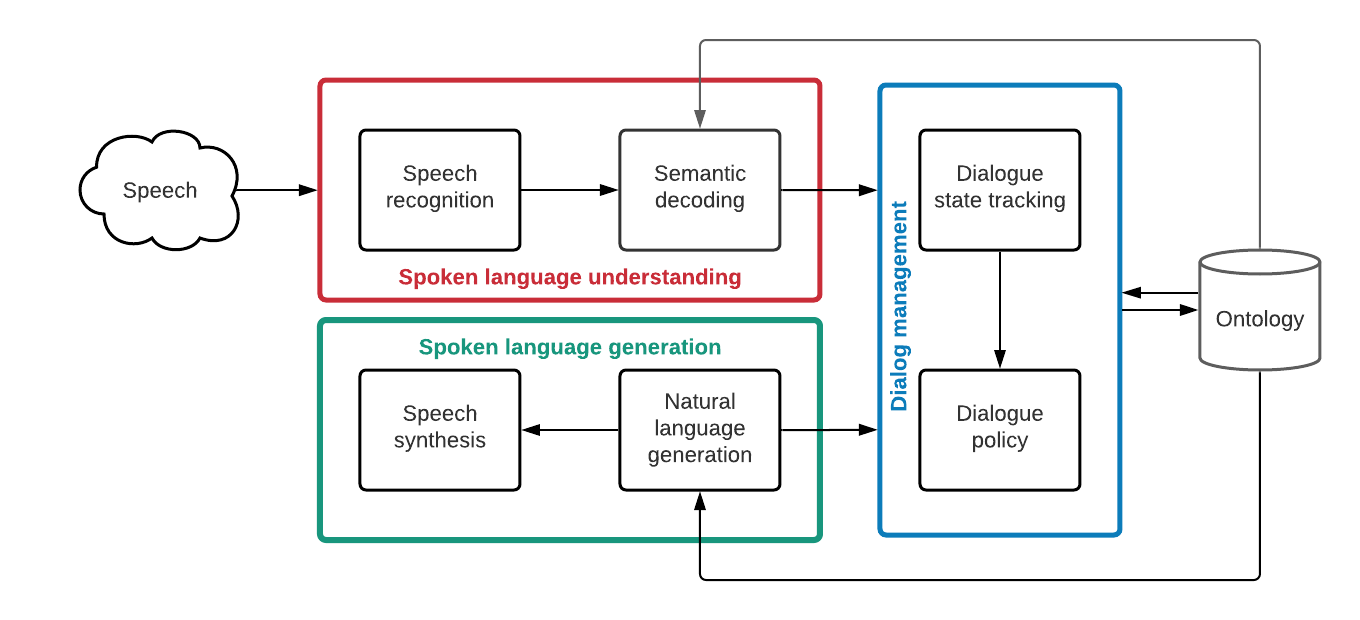
\includegraphics[width=\linewidth]{SDS-main.png}

\pagebreak
\section{Task 2 Semantic Decoding}
Semantic decoding translates sentences into the set of sematic concepts, which consists of 2 parts: intent (or dialog act type) and sematic slots and values. For instance the sentence "I want to book a flight to Berlin" can be translated into the intent "book" and the slots "flight" and "to" with the value "Berlin"($book(flight, to(Berlin))$).

To do this we first need to translate a sentence into a sequence of tags, for ex. "I want to fly from Minsk to Kiev round trip tomorrow" can be translated into the sequence of tags: ["O", "O", "O", "O", "O", "B-fromloc.city\_name", "O", "B-toloc.city\_name", "B-round\_trip", "I-round\_trip", "B-departure\_date"].

In order to do this, we can keep two dictionaries (one for words and one for tags), which will map each word (tag) to a unique integer. We can then use these dictionaries to translate the sequence of words and a sequence of tags into a sequence of integers. Then we can train a model to predict from the sequence of integers a corresponding sequence of tags. This can be a simple RNN with two heads - one for predicting the tags and another for predicting intent. 

There are different ways of how we can evaluate such model. But first, having a sequence of tags, we can convert it to a set of slots in the following way: input = [B-food-type I\_food-type O B\_price-range O], output = [(food-type, start=0, end=1), (price-range, start=3, end=3)]. Then having a set of true and predicted slots we can compare them on the slot level: if predicted slot was in true slots, then this is a true positive. If predicted slot was not in true slots, then this is a false positive. If true slot was not in predicted slots, then this is a false negative. Then from these values, we can calculate precision, recall and F1 score.

On the other hand, we can calculate accuracy directly on the predicted sequence of tags, without converting it to slots. In this case we keep the mapping of each tag to 3 counters for TP, FP and FN. After that there are 2 options on how to average the metrics. On a macro level, we first calculate precision, recall and f1-score for each of the tags, then we average these metrics across all tags. On a micro level we do the weighted average, so for ex. to calculate precision we divide the sum of all TP by the sum of all TP+FP of all tags. 

Macro average can be much lower than a weighted average, because there can be a lot of rare classes with few instances which were not predicted or predicted wrongly while there are not so many classes with a lot of instances, which are therefore predicted correctly.

Let's have a look on how the tags are recognised after training. 
\begin{center}
    \resizebox{\textwidth}{!}{
    \begin{tabular}{ c c c c c c c c c c c c c }
        & find & a & flight & from & tampa & to & montreal & by & way & of & new & york
        \\ 
        predicted & O & O & O & O & B-fromloc.city\_name & O & B-toloc.city\_name & O & O & O & B-fromloc.city\_name & I-fromloc.city\_name
        \\ 
        true & O & O & O & O & B-fromloc.city\_name & O & B-toloc.city\_name & O & O & O & B-stoploc.city\_name & I-stoploc.city\_name \\  
    \end{tabular}}
\end{center}

We can fix it by adding words "with a stop in".
\begin{center}
    \resizebox{\textwidth}{!}{
    \begin{tabular}{ c c c c c c c c c c c c c c}
        & find & a & flight & from & tampa & to & montreal & with & a & stop & in & new & york
        \\ 
        predicted & O & O & O & O & B-fromloc.city\_name & O & B-toloc.city\_name & O & O & O & O & B-stoploc.city\_name & I-stoploc.city\_name  
    \end{tabular}}
\end{center}

There are also many instances when the state name is recognized as a city name. 
\begin{center}
    \resizebox{\textwidth}{!}{
    \begin{tabular}{ c c c c c c c c c c c}
        & please & find & a & flight & from & las & vegas & to & michigan
        \\ 
        predicted & O & O & O & O & O & B-fromloc.city\_name & I-fromloc.city\_name &  O & B-toloc.city\_name
        \\ 
        true & O & O & O & O & O & B-fromloc.city\_name & I-fromloc.city\_name &  O & B-toloc.state\_name \\  
    \end{tabular}}
\end{center}

Arrival time can be mistaken with departing time:
\begin{center}
    \scalebox{0.7}{
    \begin{tabular}{ c c c c c}
        Sentence & True & Predicted & Changes & New prediction\\
        i &O&O & i & O\\
        would &O&O & would & O\\
        like  &O&O & like & O\\
        to &O& O & to & O\\
        return &O& O & fly& O\\
        from &O& O & around & B-depart\_time.time\_relative\\
        chicago &B-fromloc.city\_name& B-fromloc.city\_name & 7 & B-depart\_time.time\\
        around &B-depart\_time.time\_relative& B-depart\_time.time\_relative & in & O\\
        7 &B-depart\_time.time& B-depart\_time.time & the & O\\
        pm &I-depart\_time.time& I-arrive\_time.time & evening & B-depart\_time.period\_of\_day\\
        to &O& O & from & O\\
        kansas  &B-toloc.city\_name& B-toloc.city\_name & chicago & B-fromloc.city\_name\\
        city &I-toloc.city\_name& I-toloc.city\_name & to & O \\
        &&&kansas & B-toloc.city\_name\\
        &&& city & I-toloc.city\_name\\
    \end{tabular}}
\end{center}

We can fix wrongly recognized "pm" by adding - in the evening.
%===========================================================
\section{Task 3}
Focus tracker accumulates evidence of a changing state over the course of the dialogue. Let's define for methods and goal components $c \in V_c$ (all possible slot values) the quantity denoting that a slot(method) is not present in turn $t$:

\begin{equation}
    \label{eqn:q_c_t}
    q_{c,t} := slu_{c,t}('none') = 1 - \sum_{v \in V_c \backslash \{'none'\}}slu_{c,t}(v)
\end{equation}

\noindent where $slu(v)$ stands for 'spoken dialog undertanding' and denotes a probability of a given slot value $v$ of a goal $c$ being the correct one.\\

\noindent Let's recursively define probabilities $p_{c,t}(v)$ for each $v$ in $V_c \backslash \{'none'\}$ as: 

\begin{align}
    \label{eqn:p_c_t}
    p_{c,t}(v) &=slu_{c,t}(v) + q_{c,t} \cdot p_{c,t-1}(v) \\
    \label{eqn:p_c_0}
    p_{c,0}(v) &= slu_{c,0}(v) \\
    \label{eqn:p_c_t_none}
    p_{c,t}('none') &= 1 - \sum_{v \in V_c \backslash \{'none'\}}p_{c,t}(v)
\end{align}

\noindent For a requestable slot $s$ we define 
\begin{align}
    \label{eqn:p_s_t}
    p_{s,t} &= slu_{s,t} + (1 - slu_{s, t})\cdot p_{s,t-1} \\
    \label{eqn:p_s_0}
    p_{s,0} &= slu_{s,0}
\end{align}

\noindent Let's prove that probabilities are well-defined, in other words that $0 \leq p_{c,t}(v) \leq 1$ $\forall v \in V_c, \forall t, \forall c$

\begin{proof}
    For goals(methods).
    Using method of mathematical induction for $t=0$: \\
    From \ref{eqn:p_c_0} since $0 \leq slu_{c,t}(v) \leq 1 \implies $
    \begin{equation}
        \begin{aligned}
            0 \leq &p_{c,0}(v) \leq 1 \\
            0 \leq &p_{c, 0}('none') \leq 1
        \end{aligned}
    \end{equation}

    \noindent Assuming that probabilities are well-defined for $t = k-1$:
    \begin{equation}
        0 \leq p_{c,k-1}(v) \leq 1
    \end{equation} 
    Since
    \begin{equation}
        \begin{aligned}
            0 \leq slu_{c,k}(v) + slu_{c,k}('none') = 1 - \sum_{w \in V_{c} \backslash \{'none', v\}} slu_{c,k}(w) \leq 1
        \end{aligned}
    \end{equation}
    and
    $ slu_{c,k}(v) \geq 0 $,  $q_{c,k} \geq 0$, $p_{c,k-1}(v) \geq 0$
    then for $t=k$ we get
    \begin{equation}
        \begin{aligned}
            0 \leq p_{c, k}(v) \overset{
                \mathrm{\ref{eqn:p_c_t}}, 
                \mathrm{\ref{eqn:q_c_t}}
                }{=} slu_{c,k}(v) + q_{c,k} \cdot p_{c, k-1}(v) \leq 1
        \end{aligned}
    \end{equation}
    As $p_{c, t}('none') \leq 1$ by definition (\ref{eqn:p_c_t_none}), we only need to prove it being $\geq 0$.\\
    
    \noindent Again by method of mathematical induction let's assume that for $t = k-1$ $p_{c, k-1}('none') \geq 0$ then for $t = k$

    \begin{equation}
        \begin{aligned}
            p_{c,k}('none') 
            &\overset{
                \mathrm{\ref{eqn:p_c_t_none}},
                \mathrm{\ref{eqn:p_c_t}}, 
                \mathrm{\ref{eqn:q_c_t}}
                }{=} 1 - \sum_{v \in V_{c} \backslash \{'none'\}} \left[ slu_{c,k}(v) + q_{c,k} \cdot p_{c,k-1}(v) \right] \\ 
            &\overset{
                \mathrm{\ref{eqn:q_c_t}}
                }{=} slu_{c,k}('none') - \sum_{v \in V_{c} \backslash \{'none'\}} slu_{c,k}('none') \cdot p_{c,k-1}(v) \\ 
            &= slu_{c,k}('none')(1 - \sum_{v \in V_{c} \backslash \{'none'\}}p_{c, k-1}(v)) 
            \\
            &\overset{\sum_{V_c}p_{c, k-1}(v) = 1}{=} slu_{c,k}('none') \cdot p_{c, k-1}('none') \geq 0
        \end{aligned}
    \end{equation}

    For requestable slots.\\
    
    Assuming that probabilities are well-defined for $t = k-1$:
    \begin{equation}
        0 \leq p_{s,k-1} \leq 1
    \end{equation}
    
    Since
    
    \begin{equation}
        0 \leq slu_{s,t} + (1 - slu_{s,t}) \leq 1
    \end{equation}

    \begin{equation}
        0 \leq p_{s,t} \overset{\ref{eqn:p_s_t}}{=} slu_{s,t} + (1 - slu_{s,t}) \cdot p_{s,t-1} \leq 1
    \end{equation}
\end{proof}

\subsection{Exercise 3}
Focus tracker performes much better for the informable slots. This is an expected behaviour as informable slot may change over time, and the probability of the slot being informable will change over time. However for the requestable slot focus tracker doesn't show a better performance and usually the requestable slots do not change during the dialog, they are requested once and after that removed from the set of the requestable slots. The same applied for the methods, performance there is the similar to the baseline tracker as user only once "sets" by which method he wants to achieve the goal.

\subsection{Exercise 4}
What happens to a probability if a user gives the exact same utterance in
the first two turns of the dialog?

$slu = slu_{c, 1}(v) = slu_{c,2}(v) \Rightarrow q_{c,1} = q_{c, 2} = q$ for $\forall c \forall v \in V_c $

\begin{equation}
    \begin{aligned}
        &p_{c,2}(v) = slu_{c,2}(v) + q_c \cdot p_{c, 1}(v) 
        \\
        &p_{c,1}(v) = slu_{c,1}(v)
        \\
        &p_{c, 2}(v) = slu_{c,2}(v) + q_c \cdot p_{c, 1}(v) = slu(v)(1 + q_c)
    \end{aligned}
\end{equation}

$\Rightarrow$ probability of value $v$  for slot $c$ will grow $p_{c,2}(v) \geq p_{c,1}(v) \forall v \in V_c $

\begin{equation}
    \begin{aligned}
        p_{c,2}('none') = 1 - \sum_{v \in V_{c} \backslash \{'none'\}} p_{c,2}(v) \leq 1 - \sum_{v \in V_{c} \backslash \{'none'\}} p_{c,1}(v)  = p_{c,1}('none')
    \end{aligned}
\end{equation}

So the probability of value 'none' when the same utterance is repeated twice decreases.

\subsection{Exercise 5}
Let's defince another update rule:
\begin{equation}
    p_{c,t}(v) = (1-q_{c,t})\cdot slu_{c,t}(v) + q_{c,t} \cdot p_{c,t-1}(v)
\end{equation}
Assume we talked to the user for two turns and for an informable slot $c$ it holds that 
\begin{equation}
    \label{eqn:q_c_0_1}
    q_{c, 0} = 1
\end{equation}
and 
\begin{equation}
    \label{eqn:q_c_1}
    q_{c, 1} = slu_{c,1}(v) = 0.5
\end{equation}

\noindent What happens to the probability $p_{c,1}(v)$?\\

\noindent Since (\ref{eqn:q_c_0_1}) means that all probabilities were 0 for any $v$ apart from 'none' value, so $p_{c,0}(v) = 0$ for all $v \in V_c$ \\

\noindent Then $p_{c,1}(v) = (1 = 0.5) \cdot 0.5 + 0 = 0.25$ \\

\noindent As the slot was not in the first turn and then appeared in the second turn with probability 0.5, then it is okay to assume that the the probability of it might be not 0.5 (as it would be in previous update rule) but 0.25. \\

\noindent In general, such rule puts less weight on the new probabilities from current turn and more weight on the previous turn, which is also a totally reasonable update. 


\section{Monte-Carlo policy}

Monte Carlo control algorithm is a method for finding the optimal policy for a reinforcement problem.

\noindent It is a tabular approach, which means that the belief state/summary space is discretised into a grid. In this algorithm the policy and the Q function are first defined randomly. Then we iterate over the dialogs with this polilcy. Throught this iteration we calculate the reward until the end of the dialog. For updating the state we choose the nearest state from the table and update the Q value and afterwards the policy with it, then in the next turn we will use an already updated policy. 

\begin{center}
    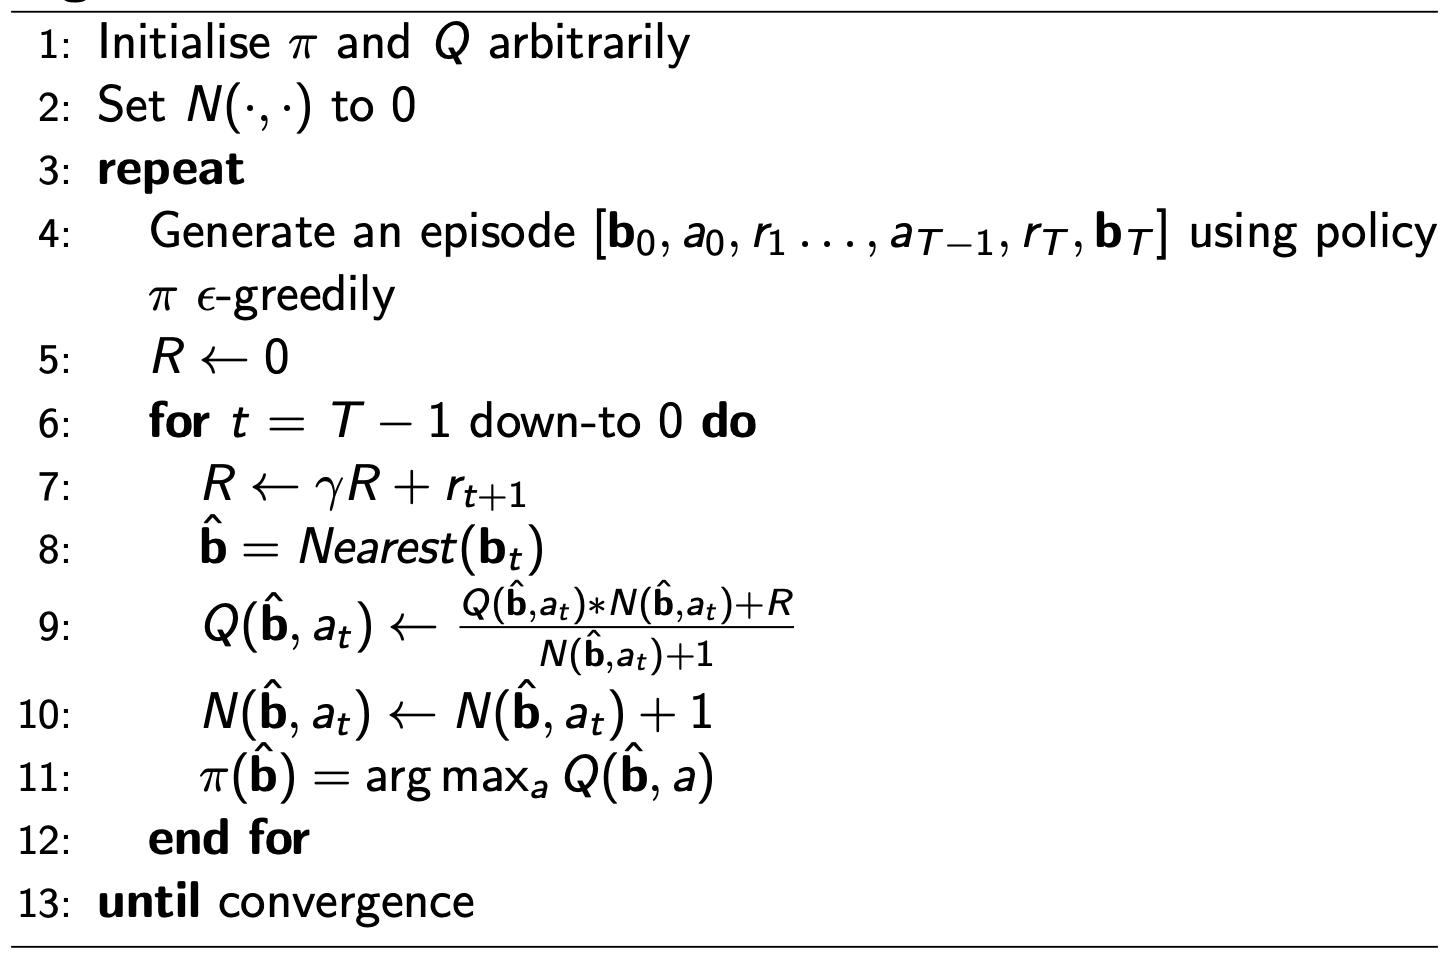
\includegraphics[width=10cm]{MCC.png}
\end{center}
It is a value-based algorithm, which means that it is based on the value of the state-action pairs. It is also a model-free method as it does not require any knowledge of the environment. And finally it is a on-policy as we use the current best estimate of the policy to guide the agent. And policy is updated iteratively until we find the optimal one. Regarding the exploration, it is a greedy method as we sometimes choose the action with the highest value, and sometimes pick a random one.

\subsection{Why do we define a reward?}

Reward is a measure of the success of the policy for the dialog, if we don’t have a reward, we cannot learn and define an optimal policy. With it we can define how we optimize the policy by optimizing the value of the reward. It is basically a metric for the algorithm's success.

\subsection{What actions can system execute?}

Interesting detail for optimizing the training process is explicitly define which actions can the system execute. This is important because we want to train the system to execute only those actions that are possible. For example, if the system is in a state where it cannot execute the action “say hello” (after user requests a restaurant's pnone number), then we should not train the system to execute that action. 

In order to implement that we can use a mask to define which actions can be executed. The mask is a binary vector of size equal to the number of actions. If the mask is 1, then the action is allowed to be executed. If the mask is 0, then the action is not allowed to be executed.

\pagebreak


%===========================================================
\section{Deep Q-Network}

%===========================================================
\subsection{Q-Learning}
Instead of keeping Q-values in a table, we keep them in a network. This network is called a Q-network. The Q-network is a neural network that takes the state of the dialog as input and outputs the Q-value for each of possible actions. The optimal Q-function (Q-network) obeys the following Bellman optimality equation: 

\[ Q*(s,a) = \E [r + \gamma max_{a^\prime}Q(s^\prime,a^\prime)] \] 

where $\gamma$ is the discount factor,  $r$ is the immediate reward and $\max_a Q(s',a)$ is the maximum Q-value of the next state. The idea of the DQN paper is to use this Bellman optimality equation to update the Q-function in an interative way:
\[Q_{i + 1} (s,a) \leftarrow \E[r + \gamma max_{a^\prime}Q_{i}(s^\prime,a^\prime)]\]
It can be shown that with these iterations we will converge to the optimal Q-function.

In comparison to Monte-Carlo approach this one is more efficient because it does not need to keep track of all the past states. Instead it only needs to keep track of the current state. This is because the Q-value of the current state is used to calculate the Q-value of the next state.

DQN approach benefints from two main ideas: experience replay and delayed Q-targets. For this type of learning the tuples of ${s, a, r, s^\prime}$, there $s^\prime$ is the following dialog state. The loss which will be minimized is the difference between the Q-value of the current state and the Q-value of the next state:

\[\L = \E_{(s, a, r, s^\prime) \sim D} [(Q_{target}(r,s^\prime) - Q(s, a))^2]\]

where $Target(r, s^\prime) = r + \gamma max_{a}Q_{target}(s^\prime,a)$

and if $s^\prime$ is a terminal state then $Q(s^\prime, a) = Q_{target}(s^\prime, a) = 0$ for every $a$.
 
As well as with Monte-Carlo we choose and $e$-greedy action selection. In this case training with the second environment is much more efficient and accurate, than training the same environment using Monte-Carlo approach. 

Experience replay provides two main advantages: first as we store data tuples $(s, a, r, s^\prime)$ in an experience buffer $D$, then each step of the experience that model encounters is potentially used in many weight updates. Second, as samples are very correlated, learning from subsequent samples is not efficient and creates a high variance.

Delayed Q-Targets means that the target network is updated with the delay, which stabilizes the network even more. The updates of the target network work as a mean-time-average?????

Additionally we have trained a Q-network without the experience replay. In this case the result was much worse and the variance was much higher, therefore the network was very unstable.

\begin{center}
    \begin{tabular}{||c c c c||} 
     \hline
      & Reward & Success & Turns \\ [0.5ex] 
     \hline\hline
     Experience replay & 11.23 +- 0.97 & 93.00 +- 3.56 & 7.37 +- 0.53 \\ 
     \hline
     No experience replay & 4.50 +- 2.04 & 69.00 +- 6.45 & 9.30 +- 0.94 \\
     \hline
    \end{tabular}
\end{center}

The same informations is presente also in the plots.

\begin{figure}[!htb]
    \minipage{0.32\textwidth}
      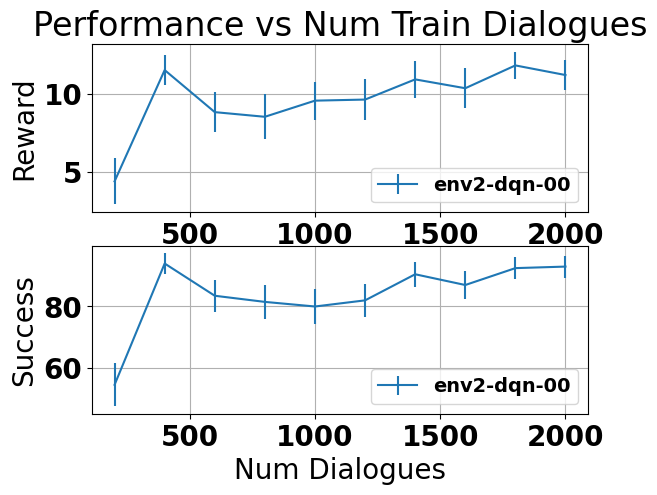
\includegraphics[width=\linewidth]{env2-CamRestaurants-experience.png}
      \caption{Experience Replay}
    \endminipage\hfill
    \minipage{0.32\textwidth}
      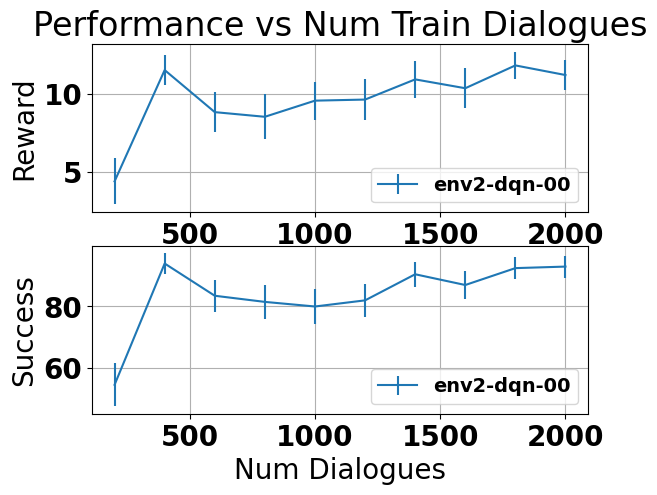
\includegraphics[width=\linewidth]{env2-CamRestaurants-experience.png}
      \caption{No Experience Replay}
    \endminipage\hfill
    \minipage{0.32\textwidth}%
      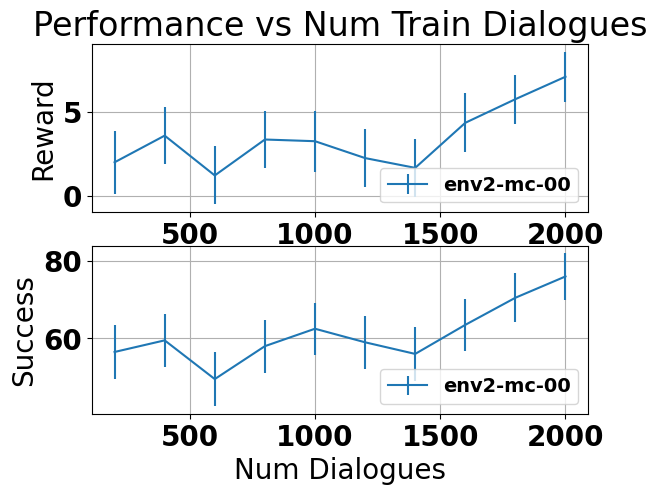
\includegraphics[width=\linewidth]{env2-CamRestaurants-mc.png}
      \caption{Monte-Carlo}
    \endminipage
\end{figure}

As the system is not supposed to live on its own, here we present several dialogs conducted with it. 
%=========================================================== 
\section{Zweiter Abschnitt}

However, these methods were previously quite unstable (Mnih et al., 2013). In DQN,
Mnih et al. (2013, 2015) proposed two techniques
to overcome this instability-namely experience replay and the use of a target network. In experience replay, all the transitions are put in a finite
pool D (Lin, 1993). Once the pool has reached
its predefined maximum size, adding a new transition results in deleting the oldest transition in
the pool. During training, a mini-batch of transitions is uniformly sampled from the pool, i.e.
(Bt
, At
, Rt+1, Bt+1) from U(D). This method removes the instability arising from strong correlation between the subsequent transitions of an
episode (a dialogue). Additionally, a target network with weight vector w is used. This target
network is similar to the Q-network except that
its weights are only copied every tau steps from the
Q-network, and remain fixed during all the other
steps. The loss function for the Q-network at iter

\pagebreak
\begin{thebibliography}{ccccc}
\addcontentsline{toc}{section}{Literatur}

%So kann eine eine Monographie zitieren:
\bibitem{Arbarello et al 1985}
E.\ Arbarello, M.\ Cornalba, P.\ Griffiths, J.\ Harris:
Geometry of algebraic curves. I. 
Springer, New York, 1985.

%So kann man eine Originalarbeit zitieren:
\bibitem{Shepherd-Barron 1997}
N.\ Shepherd-Barron:
Fano threefolds in positive characteristic.
Compositio Math.\  105  (1997),  237--265.

\end{thebibliography}



%===========================================================
\pagebreak\noindent
\textbf{\LARGE Erkl\"arung}
\addcontentsline{toc}{section}{Erkl\"arung}

\bigskip\bigskip
\noindent 
Hiermit versichere ich, dass ich die   Bachelorarbeit selbst\"andig verfasst und keine
anderen als die angegebenen Quellen und Hilfsmittel benutzt habe.

\bigskip
\noindent
D\"usseldorf, den tt.\ Monat jjjj

\bigskip\bigskip\bigskip
\noindent
(Vorname Nachname)

\end{document}